\chapter{Operations \& Logistics}
\label{sec:ol}
%introduction
In this chapter the operational and logistical aspects of the design will be evaluated provisionally. It is not part of the trade-off concept since all concepts share the same procedures and infrastructure, but is intended to serve as preparation for the detailed design phase. A flow diagram describing support facilities, equipment and activities is included, as well as considerations on the mission operation itself.  

\section{Ground operations and logistics}

\begin{figure}[htb]
    \centering
    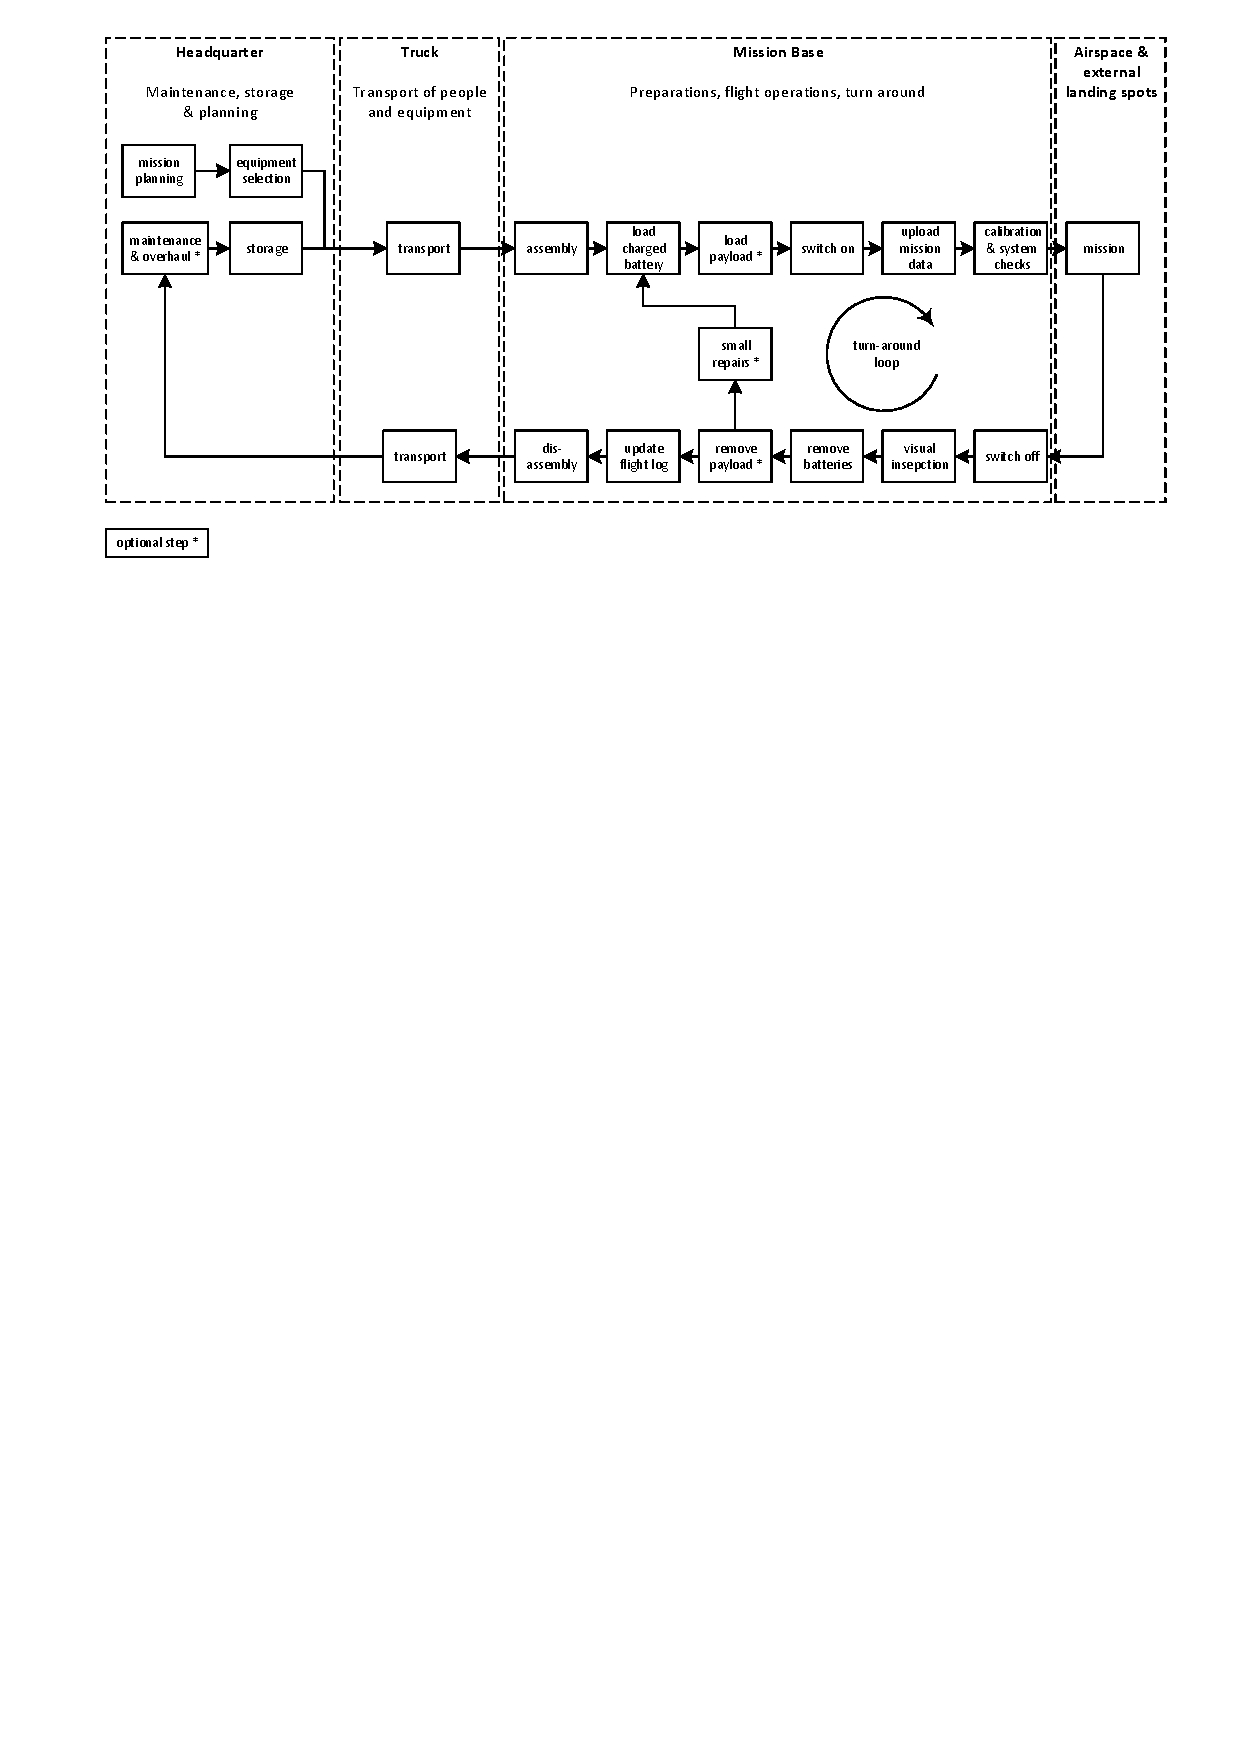
\includegraphics[width=1.05\textwidth]{Operations/Figures/operations_logistics.pdf}
    \caption{Operations \& logistics flow diagram}
    \label{fig:opslogsdig}
\end{figure}

\autoref{fig:opslogsdig} shows the the operations and logistics flow diagram for what this group expects to be typical operating conditions. It is assumed that the UAV operator has a main facility, from which the UAV, staff and mission relevant equipment are transported to a mission base at which flight operations take place. Naturally, variations to this scheme are possible, e.g. a parcel company may exclusively operate from its main facility, or long-range missions require a turn-around at a remote location, but for the sake of brevity only the most general case is presented.
The starting and end points of each mission are the so-called 'headquarters', the place where maintenance and storage takes place. Based on customer input a mission plan is set up, which determines the kind of resources that are required. Next to one or more UAVs, this includes staff on site, equipment such as the ground station, spare parts, additional batteries and a transport vehicle. Once the preparation is done, everything is loaded into a vehicle and transported to the location where the UAV is intended to take off and land. On site, the equipment needs to be unloaded and the UAV assembled into its operational form. A charged battery is then loaded, followed by the payload, which can also consist of another set of batteries. The system is switched on, the mission relevant data is uploaded to the on-board computer and an automated instrument calibration and readiness check performed. The UAV is now ready to fly and carry out its mission. After its return, the system is switched off for safety reasons, visually inspected and stripped off its batteries. The next steps depend on the kind of mission in question. If another flight is scheduled, the payload can be replaced and minor repairs taken out, e.g. replacing a damaged propeller blade. Once the battery is recharged or replaced by a full one, a new flight cycle can start. In case the mission does not comprise a turn-around or substantial damage was detected, the digital flight log is updated and the UAV disassembled. After loading all equipment the transport back to the headquarter takes place, where scheduled maintenance and all levels of repairs are carried out. Once the work is documented and approved, the equipment is stored and ready for the next mission. 


\section{Flight operations}

The amount of human interaction in flight operations varies depending on future regulations on what level of autonomy will be allowed. Current regulations only allow for operations within visual line of sight, which means that a pilot has to be able to see the UAV at all times and take control from automated systems immediately. While this is acceptable for certain mission profiles, the high range and speed of the UAV make it ideal for distances beyond visual line of sight. There are two different approaches towards BVLOS operations, which both have advantages and disadvantages. The first one is full autonomy of the UAV, meaning that once the mission data is uploaded and the system cleared for take-off, there is no further need for human interaction and therefore a data link. While this decreases the workload for ground staff, there are a number of drawbacks. First of all, the system has to be safe under all conditions. Being both fast and heavy means it poses a risk to people both in the air and on the ground, so advanced algorithms would be required to deal with abnormal conditions and emergency situations. Certification is therefore likely to be a tedious and expensive process, unless operations are exclusively performed in restricted airspace and over sparsely populated areas. Secondly, data links can not only be used for supervision and control, but also for real-time information. Certain missions might require constant transmission of video data and en-route changes of the flight path, others have customers that are very interested in the well-being of their parcel. From a technical point of view, the UAV requires a variety of sensors such as accelerometers, gyroscopes, stereoscopic cameras and lasers, and also an on-board computer able to process the incoming data and take the appropriate action. Results are increased weight, complexity and also cost.

The other option for BVLOS operations is a constant data-link to the ground station, with the option of manual control. While this kind of system also needs to demonstrate its safety, it is a lot easier to achieve in the near future and can serve as an intermediate step to full autonomy. Basic and tedious tasks such as following way points or extended surveillance can be automated, while more complex ones like landing on difficult terrain are left to a human operator. \autoref{ch:layo_and_conf} features an overview of the UAV's communications architecture, including a satellite link and cellular connection.

\section{Ground station}

The selection of a ground station is part of the next project phase but it is already possible to derive certain properties from the logistics and flight operation description:

\begin{itemize}
    \item briefcase-like shape with computing unit, screen, keyboard, trackball, 4-axis joystick and throttle
    \item on-screen information: camera feed, standard flight instruments, system status, navigation; other information on demand
    \item external antenna with wired connection
    \item redundant batteries for uninterrupted power supply
\end{itemize}

\autoref{fig:generic_gs} shows a commercial, portable ground station as is intended for the Hybrid UAV\footnote{\url{http://www.directindustry.com/prod/birdpilot-gmbh/product-162555-1691159.html}}.

\begin{figure}[htb]
    \centering
    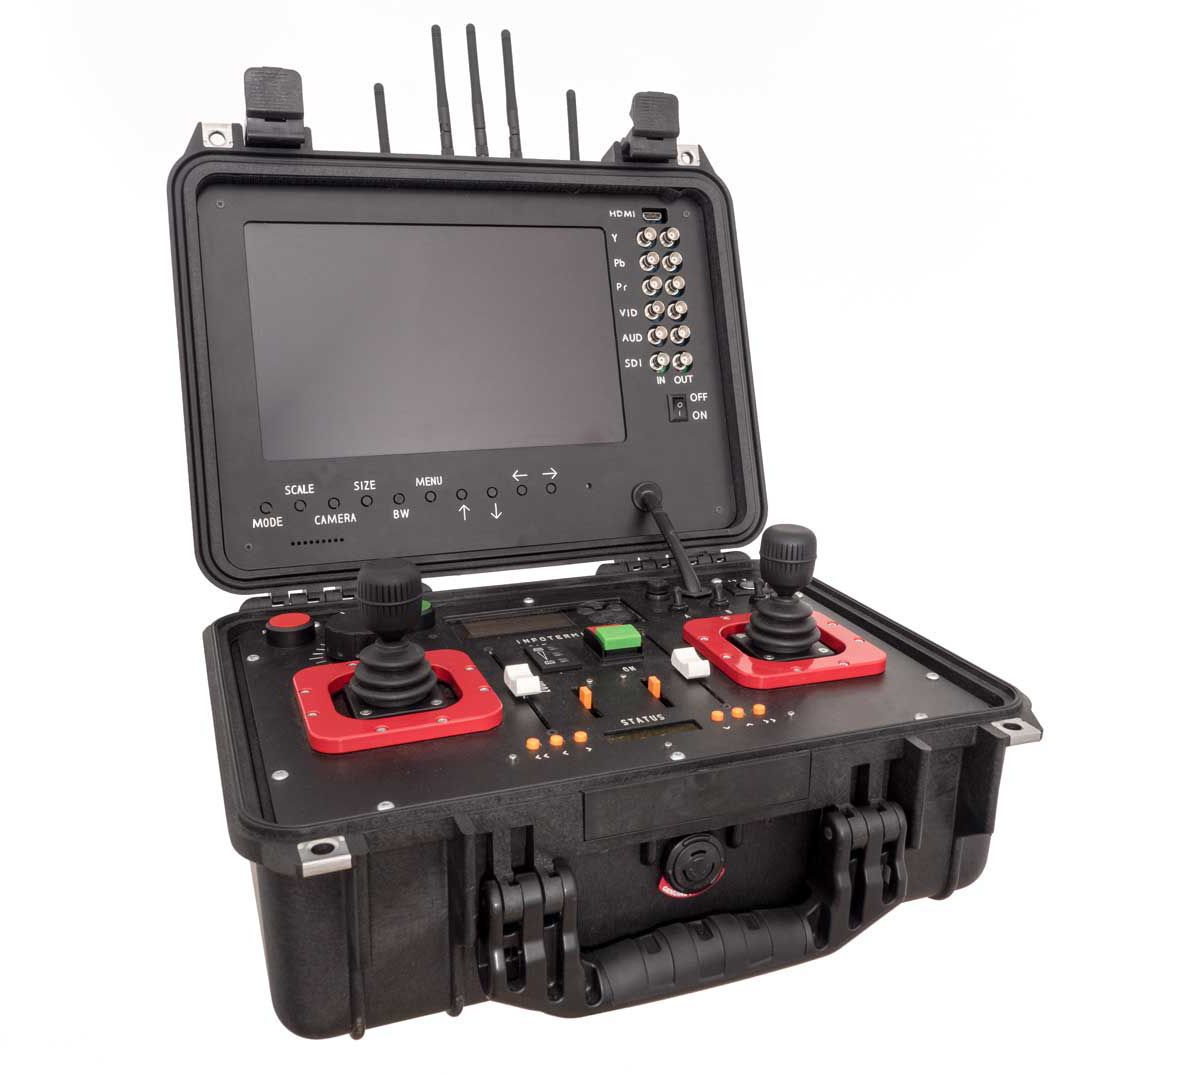
\includegraphics[width=0.5\textwidth]{Operations/Figures/ground.jpg}
    \caption{Portable UAV ground station}
    \label{fig:generic_gs}
\end{figure}